%!TEX root = Thesis.tex
\chapter{Implementation and Evaluation}
The chapter presents a prototype of the reference scenario considered in the section
2.3. The prototype implements the major aspects proposed in the concept (chapter
4).
%%%%%%%%%%%%%%%%%%%%%%%%%%%%%%%%%%%
\section{Overview of Framework}
\section{Web-based Framework Analysis}
 \begin{itemize}
\item \textbf{Bootstrap}
\newline
Bootstrap is the most popular and widely used framework, nowadays. It’s a beautiful, intuitive and powerful web design kit for creating cross browser, consistent and good looking interfaces. It offers many of the popular UI components with a plain-yet-elegant style, a grid system and JavaScript plugins for common scenarios.

It is built with LESS and consists of four main parts:
Scaffolding – global styles, responsive 12-column grids and layouts. Bear in mind that Bootstrap doesn’t include responsive features by default. If design needs to be responsive this functionality have to be done manually.
Base CSS – this includes fundamental HTML elements like tables, forms, buttons, and images, styled and enhanced with extensible classes.
Components – collection of reusable components like dropdowns, button groups, navigation controls (tabs, pills, lists, breadcrumbs, pagination), thumbnails, progress bars, media objects, and more.
JavaScript – jQuery plugins which bring the above components to life, plus transitions, modals, tool tips, popovers, scrollspy (for automatically updating nav targets based on scroll position), carousel, typeahead (a fast and fully-featured autocomplete library), affix navigation, and more.
\item \textbf{Foundation}
\newline
Foundation is a powerful, feature-rich, responsive front-end framework. With Foundation user can quickly prototype and build websites or apps that work on any kind of device, with tons of included layout constructs, elements and best practices. It’s built with mobile first in mind, utilitizes semantic features, and uses Zepto instead of jQuery in order to brings better user experience and faster performance.

Foundation has a 12-column flexible, nestable grid powerful enough to create rapidly multi-device layouts. In terms of features it provides many. There are styles for typography, buttons, forms, and various navigation controls. Many useful CSS components are provided like panels, pricing tables, progress bars, tables, thumbnails, and flex video that can scale properly your video on any device. And, of course, JavaScript plugins including dropdowns, joyride (a simple and easy website tour), magellan ( a sticky navigation that indicates where is the user on the page), orbit (a responsive image slider with touch support), reveal (for creating modal dialogs or pop-up windows),  sections (a powerful replacement for traditional accordions and tabs), and tooltips.
\item \textbf{GroundworkCSS}
\newline
GroundworkCSS is a new, fresh addition to the front-end frameworks family. It’s a fully responsive HTML5, CSS and JavaScript toolkit built with the power of Sass and Compass which gives the ability to rapidly prototype and build websites and apps that work on virtually any device.

It offers an extremely flexible, nestable, fraction-based, fluid grid system that makes creating any layout possible. GroundworkCSS has some really expressive features like tablets and mobile grids which maintain the grid column structure instead of collapsing the grid columns into individual rows when the viewport is below 768 or 480 pixels wide. Another cool feature is a jQuery ResponsiveText plugin which allows to have dynamically sized text that adapts to the width of the viewport: extremely useful for scalable headlines and building responsive tables.
The framework includes a rich set of UI components like tabs, responsive data tables, buttons, forms, responsive navigation controls, tiles (a beautiful alternative to radio buttons and other boring standard form elements), tooltips, modals, Cycle2(a powerful, responsive content slider), and many more useful elements and helpers. It also offers a nice set of vector social icons and a full suite of pictographic icons included in FontAwesome.
To see the framework in action user can use the resizer at the top center of the browser window. This way user can test the responsiveness of the components against different sizes and viewports while exploring the framework’s features.
GroundworkCSS is very well documented with many examples, and to get user started quickly the framework also provides several responsive templates. The only thing as a weakness is the missing of a way to customize download.

\item \textbf{Gumby}            
\newline
Gumby is simple, flexible, and robust front-end framework built with Sass and Compass.

Its fluid-fixed layout self-optimizes the content for desktop and mobile resolutions. It support multiple types of grids, including nested ones, with different column variations. Gumby has two PSD templates that get user started designing on 12 and 16 column grid systems.
The framework offers feature-rich UI Kit which includes buttons, forms, mobile navigation, tabs, skip links, toggles and switches, drawers, responsive images, retina images, and more. Following the latest design trends the UI elements have Metro style flat design but can use Pretty style with gradient design too, or to mix up both styles. An awesome set of responsive, resolution independent Entypo icons, is completely integrated into the Gumby Framework. Gumby has also a very good customizer with color pickers which helps to build your custom download with ease.
\item \textbf{Kube}
\newline
Lastly, if user need a solid, yet simple base without needless complexity and extras, for your new project, Kube can be the right choice. Kube is a minimal, responsive and adaptive framework with no imposed styling which gives to user the freedom to create. It offers basic styles for grids, forms, typography, tables, buttons, navigation, and other stuff like links or images.

The framework contains one compact CSS file for building responsive layouts with ease and two JS files for implementing tabs and buttons in your designs. If user is looking for maximum flexibility and customization, user can download developer version which includes LESS files, with variables, mixins and modules.
\end{itemize}

\begin{figure}[!ht]
\centering
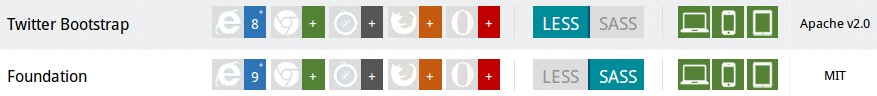
\includegraphics[scale=0.7]{images/Bootstrap&Foundation.png}
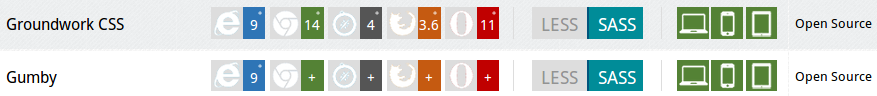
\includegraphics[scale=0.7]{images/Groundwork&Gumby.png} 
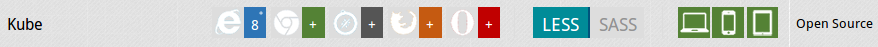
\includegraphics[scale=0.7]{images/Kube.png}  
\caption[Framework Comparison]{Framework Comparison\footnote{\url{http://usablica.github.io/front-end-frameworks/compare.html}}}
\label{img:Bootstrap&Foundation.png}
\label{img:Groundwork&Gumby.png}   
\label{img:Kube.png}                          
\end{figure}
\section{Data Flow Model}
\section{Model-View-Control Pattern}
In the design shown in Figure 1 on page X Model represents the application
object that implements the application data and business logic. The View is
responsible for formatting the application results and dynamic page construction.
The Controller is responsible for receiving the client request, invoking the
appropriate business logic, and based on the results, selecting the appropriate
view to be presented to the user.
The Model represents enterprise data and the business rules that govern
access to and updates to this data. Often the Model serves as a software
approximation to a real-world process, so simple real-world modeling
techniques apply when defining the Model.
A View renders the contents of a Model. It accesses enterprise data through
the Model and specifies how that data should be presented.
It is the View's responsibility to maintain consistency in its presentation when
the Model changes. This can be achieved by using a push Model, where the
View registers itself with the Model for change notifications, or a pull Model,
where the View is responsible for calling the Model when it needs to retrieve
the most current data.
A Controller translates interactions with the View into actions to be performed
by the Model. In a stand-alone GUI client, user interactions could be button
clicks or menu selections, whereas in a Web application, they appear as GET
and POST HTTP requests. The actions performed by the Model include
activating business processes or changing the state of the Model. Based on
the user interactions and the outcome of the Model actions, the Controller
responds by selecting an appropriate View.
\begin{figure}[!ht]
\centering
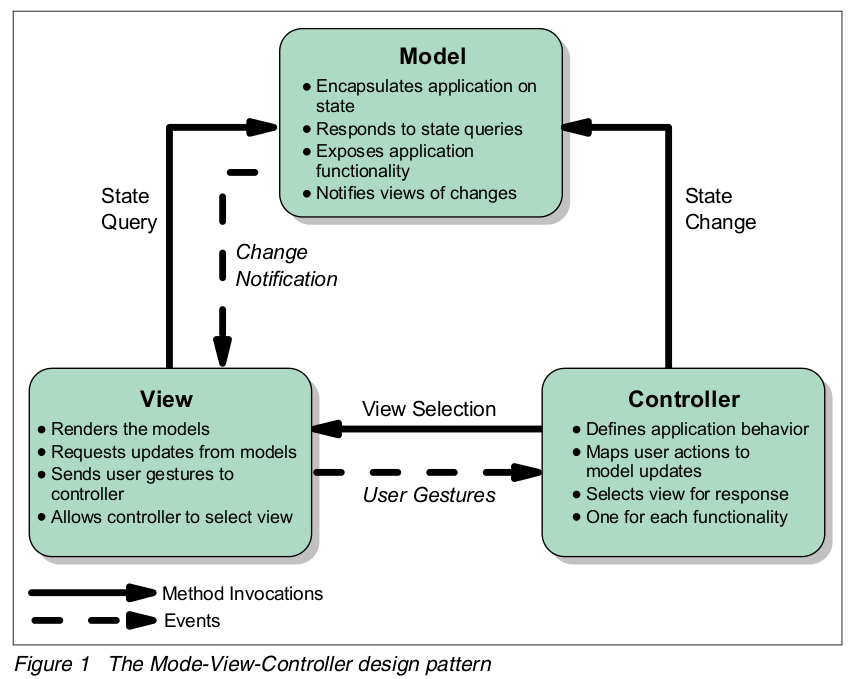
\includegraphics[scale=0.5]{images/MVCPattern.png}   
\caption[MVC Pattern]{MVC Pattern}
\label{img:MVCPattern}                           
\end{figure}
\section{Database Model}
\section{Use Cases}
  \subsection{Frontend}
  \subsection{Choosen Environment}
  \subsection{Choosen Tools}
  \subsection{Use Cases Realization}
\subsection{Summary}